\documentclass[10pt, preprint]{sigplanconf}

% The following \documentclass options may be useful:

% preprint      Remove this option only once the paper is in final form.
% 10pt          To set in 10-point type instead of 9-point.
% 11pt          To set in 11-point type instead of 9-point.
% authoryear    To obtain author/year citation style instead of numeric.

\usepackage{amsmath}
\usepackage{amssymb}
\usepackage{listings}
\usepackage{hyperref}
\usepackage{subcaption}
\usepackage{todo}

\special{papersize=8.5in,11in}
\setlength{\pdfpageheight}{\paperheight}
\setlength{\pdfpagewidth}{\paperwidth}

\lstset{captionpos=b, float, language=python}

\usepackage{tikz}
\usetikzlibrary{positioning}
\usetikzlibrary{shadows}
\usetikzlibrary{arrows}
\usetikzlibrary{shapes}
\usetikzlibrary{calc}

\providecommand{\boostsimd}{\textsc{Boost.SIMD}}
\providecommand{\cpp}[1][~]{\textsc{C++}#1}
\providecommand{\ie}[1][~]{\textit{i.e.}#1}
\providecommand{\eg}[1][~]{\textit{e.g.#1}}


\begin{document}


\title{Efficient Compilation of High Level Python Numerical Programs with Pythran}

\authorinfo{Serge Guelton}
           {T{\'e}l{\'e}com Bretagne}
           {serge.guelton@telecom-bretagne.eu}
\authorinfo{Pierrick Brunet}
           {INRIA/MOAIS}
           {pierrick.brunet@inria.fr}
\authorinfo{Mehdi Amini}
           {SILKAN}
           {mehdi.amini@silkan.com}

\maketitle

\begin{abstract}

    For decades, FORTRAN and C(++) have dominated the landscape of High
    Performance Computing languages, leaving interpreted language like Matlab,
    R, Python or more recently Julia for experimentation and prototyping.

    As more scientists use these scripting languages, there is an on-going
    research effort to compile them into efficient native code. However as
    these languages favor a high-level coding style, the computation kernels are
    different from what we use to see in traditional C or Fortran programs:
    explicit raw loops are replaced by high-level constructs and calls to the
    relevant toolbox/module/library/package. As a consequence, traditional
    algorithms to perform
    loop optimization techniques like fusion, tiling and related
    vectorization or parallelization techniques are not directly applicable.

    This papers focuses on the case of the Python language and especially the
    Numpy package that provides core array data structure and basic linear
    algebra routines. It first conducts a case study based on Numpy use
    cases from the StackOverflow question and answer website, then studies
    existing compilers for numerical Python. Optimization opportunities,
    including parallelization and vectorization, and their implementation in
    the Pythran compiler are presented and illustrated through several
    benchmarks, showing very interesting speedups over the standard Python
    interpreter. Speedup greater than a factor of 10 are achieved despite the
    fact that the considered benchmarks mostly call Numpy routines that run C code.

\end{abstract}


\keywords
Static Compilation, Parallelization, Python, C++, SIMD, Runtime

%%
%%
\section{Introduction}
% On aura pas le temps pour le papier je pense mais faire une comparaison avec
% du C pure pour voir ce que les compilo de C arrive a faire.

The Python language~\cite{rossum97} has a rich ecosystem that now provides a
full toolkit to carry out scientific experiments, from core scientific routines
with the Numpy package\cite{oliphant2007,numpyarray2011}, to scientific
packages with the Scipy package~\cite{scipy}, plotting facilities with the
Matplotlib package, enhanced terminal and notebooks with IPython. As a
consequence, there has been a move from historical languages like Fortran to
Python, as showcased by the success of the Scipy conference.

As Python based scientific tools gets widely used, the question of High
performance Computing naturally arises, and it is the focus of many recent
research. Indeed, although there is a great gain in productivity when using
these tools, there is also a performance gap that needs to be filled.

This paper focuses on compilation techniques that are relevant for the
optimization of high-level numerical kernels written in Python using the Numpy
package. Its shows an implementation of these techniques through the Pythran
compiler and provided a benchmarks test suite for performance measures with
others Python compilers.
Section~\ref{sec:stackoverflow} presents a case study based on user
input gathered on the StackOverflow question and answer site.
Section~\ref{sec:optimize} focuses on a simple yet representative kernel and
showcases the optimization opportunities typically found in Numpy-based
kernels. Existing compilation approach to optimize such kernels are discussed
in Section~\ref{sec:compilers}, then Section~\ref{sec:pythran} emphasises on a
compiler-runtime cooperative approach to solve the performance issues.
Experimentations showcasing important performance gains are detailed in
Section~\ref{sec:xp}.


%%
%%
\section{A Crowd-Sourced Numpy Benchmark}
\label{sec:stackoverflow}

One of the first steps required when designing an optimizing compiler is to
gather enough test cases, or benchmarks, in order to drive the optimization
process toward realistic examples. To achieve this goal, we have gathered a few
examples from existing compilers' test suite, but these may have been modified to
overcome some compiler limitations. A less biased source of benchmarks should
be independent from the compiler community and focused on matching user needs.
To achieve that goal, we collected synthetic scientific kernels from the
StackOverflow website.

StackOverflow~\footnote{\url{http://stackoverflow.com/}} is a question and
answer site for programmers. Any registered user can submit questions and other
users may answer. A voting system is then used to sort the answers. Said
otherwise, the website provides a database of question and answers on
programming topics, including Python.

A query using the terms \emph{numpy} and \emph{slow} yields a lot of results, many
of which use the pattern ``Q: my code is slow'' followed by an upvoted answer
``A: rewrite it that way'', where the original code performs explicit looping
over an array, and the rewritten code uses the relevant combination of Numpy
function.

For instance, question \href{http://stackoverflow.com/questions/7741878}{7741878}
proposes to use an explicit loop to iteratively compute the $L^2$ norm of each
row of a matrix, as illustrated in Listing~\ref{lst:l2norm-loopy}, and one of
the proposed answer is to use the more compact version presented in
Listing~\ref{lst:l2norm}. This answer no longer uses any explicit loops and
roughly achieves a $\times 4$ speedup over the loop version.

\begin{lstlisting}[language=python,caption={Per row version of $L^2$ norm with loop in Numpy.}, label={lst:l2norm-loopy}]
def slow(x):
    r = np.empty(x.shape[0])
    for i in xrange(x.shape[0]):
        r[i] = np.sum(np.abs(x[i])**2)
    return r
\end{lstlisting}

\begin{lstlisting}[language=python,caption={Per row version of $L^2$ norm without loop in Numpy.}, label={lst:l2norm}]
import numpy as np
def l2norm(x):
    return np.sum(np.abs(x)**2, axis=1)
\end{lstlisting}

Newcomers to Python with a prior C or Fortran experience are likely to make
use of raw loops similar to Listing~\ref{lst:l2norm-loopy}, but as their
command of the Numpy API and of good programming practices grows, they get to write code similar
to Listing~\ref{lst:l2norm}. The fact that in Numpy, high-level constructs run faster is also a
strong motivation. As a direct consequence, a compiler should focus on optimizing
high-level constructs rather than raw
loops. Both to encourage good practice with respect to Numpy code, and because
this is the kind of code Numpy users ultimately write.

The benchmarks collected during this process are publicly available on
\url{https://github.com/serge-sans-paille/numpy-benchmarks}, with a set of
benchmarking routine specialized for major Python/Numpy compilers.


%%
%%
\section{Optimizations Opportunities in a Typical Numpy Kernel}
\label{sec:optimize}

Let us consider the kernel illustrated in Listing~\ref{lst:rosen} and adapted
from the Scipy source code of \texttt{scipy.optimize.rosen}. This kernel makes
use of Numpy's \texttt{sum} function, Python's square notation and Numpy's
array slicing. It is a good example of high-level Python kernel, although
using the function \texttt{scipy.optimize.rosen} directly would naturally make sense.

\begin{lstlisting}[language=python, caption={High-level implementation of the Rosenbrock function in Numpy.}, label={lst:rosen}]
def rosen(x):
    t0 = 100 * (x[1:] - x[:-1] ** 2) ** 2
    t1 = (1 - x[:-1]) ** 2
    return numpy.sum(t0 + t1)
\end{lstlisting}

This section goes through all the optimization opportunities in
Listing~\ref{lst:rosen} as a showcase of what an optimizing compiler could do.


\subsection{Temporaries Elimination}
\label{sec:temporaries-elimination}

In Numpy, all point-to-point array operations allocate a new array that holds
the computation result. This behavior is consistent with many Python standard
module, but it is a very inefficient design choice, as it keeps on polluting
the cache with potentially large fresh storage and add an extra
allocation/deallocation costly operation. In the \textit{rosen} function from
Listing~\ref{lst:rosen}, 7 temporary arrays are allocated (slicing does not
create a temporary array but a view) to hold intermediate steps. Had the
computation been lazy, no temporary would have been needed.

\subsection{Operator Fusion}
\label{sec:operator-fusion}

As Numpy is a native library mostly written in C, each operator computation is
performed by a function implemented as a loop performing a single operation,
and the operator chaining is done at the interpreter level. This is a typical
problem in library design: if only a small set of functions is provided, it
prevents the optimization of merging multiple operators into a single specialized
operator, and provided many operator combinations as part of the library yields
better performance to the price of API bloat. The Listing~\ref{lst:rosen}
illustrates the use of a small set of functions: a loop is used for
each temporary computation, plus an extra loop for the \texttt{numpy.sum}
reduction, where a single loop would have been needed with operator fusion.

\subsection{Loop Vectorization and Parallelization}

Without operator fusion, there would be very little benefit to generate SIMD
instructions for the respective array operations used by each operator, as the
memory load and store would have dominated the execution time. This is even more important as
Numpy typically operates on double precision floats, which means only two (SSE)
to four (AVX) scalar per vector registers.

Parallelization also suffers from the lack of operator fusion: a
synchronization fence is needed between each temporary computation.  Hence the
loop computation intensity would be very low compared to the memory pressure
implied by two array reads and one array write for a single binary operator.

On the opposite, if all computations were merged into a single loop using
temporaries elimination and operator fusion, parallelization would be more
effective as barrier between binary operations are no longer needed and loads
and stores will be used to perform multiple operations.

%%
%%
\section{Existing Compilation Approach}
\label{sec:compilers}

The success of Python and the development of its large ecosystem triggered
several attempts to improve its execution speed. The most significant basic
block for high performance numerical simulations is certainly Numpy, a
numerical library to manipulate dense arrays. However, this library-like
approach has inherent limitations that have been exposed in \S~\ref{sec:optimize}.
To address these limitations, several compiler-based approaches have been proposed.

\subsection{Numpy}

The reference implementation of Numpy is a native Module, written mostly in C.
It uses the BLAS API whenever possible and provides a relatively efficient array
abstraction in the form of the \texttt{ndarray} data structure. This data
structures makes it possible to use various styles of slicing and broadcasting,
as illustrated in Listing~\ref{lst:pairwise}.

It also enforces a high-level programming style but it's very inefficient when
explicit subscripts are used.  For instance, raw loops are used in
Listing~\ref{lst:pairwise-raw}. It avoids the creation of temporary arrays but
runs almost 100 times slower due to the Python interpreter overhead and the C
to Python conversion involved in every subscript.

\begin{lstlisting}[language=python, caption={\textit{pairwise} function that
  exhibits array broadcasting.}, label={lst:pairwise}, breaklines=true]]
def pairwise_numpy(X):
    return np.sqrt(((X[:, None, :] - X) ** 2).sum(-1))
\end{lstlisting}


\begin{lstlisting}[language=python, caption={\textit{pairwise} function
  using raw loops.}, label={lst:pairwise-raw}]
def pairwise_python(X):
    M = X.shape[0]
    N = X.shape[1]
    D = np.empty((M, M), dtype=np.float)
    for i in range(M):
        for j in range(M):
            d = 0.0
            for k in range(N):
                tmp = X[i, k] - X[j, k]
                d += tmp * tmp
            D[i, j] = np.sqrt(d)
    return D
\end{lstlisting}

\subsection{Cython}
%
Cython~\cite{cython2010} is an hybrid Python/C dialect. It extends the Python
syntax with typing information, calls to native functions from third party C
libraries, and a limited set of parallelism constructs, such as the possibility
to define parallel loops, but no task parallelism. When possible, it unboxes % ref?
Python variables to improve performance. Without type annotations, the
performance improvement is not significant, but given enough type annotation,
Cython can generates code that runs as fast as its C equivalent.

The drawback is that the programmer has to avoid high-level constructs and
instead expresses his algorithm using raw loops.  The \textit{pairwise}
function rewritten for Cython is shown listing~\ref{lst:pairwise-cython},
showing usage of compiler annotations in the form of function decorators.

\begin{lstlisting}[language=python, caption={\textit{pairwise} function
  rewritten for Cython.}, label={lst:pairwise-cython}]
%%cython
import numpy as np
cimport cython
from libc.math cimport sqrt

@cython.boundscheck(False)
@cython.wraparound(False)
def pairwise_cython(double[:, ::1] X):
 cdef int M = X.shape[0]
 cdef int N = X.shape[1]
 cdef double tmp, d
 cdef double[:, ::1] D
 D = np.empty((M, M), dtype=np.float64)
 for i in range(M):
  for j in range(M):
   d = 0.0
    for k in range(N):
     tmp = X[i, k] - X[j, k]
     d += tmp * tmp
    D[i, j] = sqrt(d)
 return np.asarray(D)
\end{lstlisting}

\subsection{Numba}


The Numba compiler uses additional type information collected at run-time to
generate sequential LLVM bytecode.  Numba uses Just-In-Time(JIT) compilation
and does not suffer from backward-incompatibility issues: a single
\texttt{@jit} decorator is used to flag kernels to optimize. When meeting an
unsupported construct, Numba silently falls back to Python C-API calls.

Like Python, Numba is providing its best speedup on code with raw loops, which
is not encouraging programmers to express their code using the higher-level
construct available with Numpy. However, when input constraint are met, it
exhibits performance close to Cython, or even better when conversion to GPU
code is possible.

\subsection{Parakeet}

Parakeet~\cite{parakeet2012} follows an approach similar to Numba, that is JIT
compilation of selected kernels. It uses C annotated with OpenMP directives as
a target language, but limits its scope to the Numpy package, only supporting
the subset of the Python language required to use Numpy functions.
Additionally, it supports implicit parallelism using an implicit mapping
between Numpy functions and a set of parallel primitives including
\texttt{map}, \texttt{scan}, and \texttt{reduce}.  As it applies optimizations
such as operator fusion, it encourages programmer to express their code using
the higher-level construct available with Numpy.

\subsection{Copperhead}

Copperhead~\cite{copperhead2011} is a functional, data parallel language
embedded in Python. It uses $n$-uplets, Numpy arrays and lists as its core data
structure and prohibits usage of many control-flow operators such as loops,
enforcing the use of the \texttt{map}, \texttt{filter} or \texttt{reduce}
intrinsics to exhibit parallelism. But it can be efficiently compiled to either
CUDA or C++ with calls to the Thrust\footnote{\emph{cf}.
\texttt{http://thrust.github.com/}} library. Like Numba and Parakeet, it uses
Python decorators to identify hot-spots that are JIT-compiled to native code.
As it requires to write functional code, it is not compatible with the Numpy
interface, although several Numpy functions could be rewritten in terms of
Copperhead intrinsics.

\subsection{PyPy and Shed~Skin}

PyPy~\cite{pypy2009}, a fully compatible Python interpreter with a tracing JIT,
or Shed~Skin~\cite{shedskin2006}, a Python to C++ compiler, are also viable
ways to enhance Python performance. However Shed~Skin does not provide support
for the Numpy module. PyPy faces the issue of calling native libraries that
cannot be optimized by a Python JIT compiler. There is an important work in
progress from the community to support Numpy, but it implies a partial rewrite
of the Numpy API in RPython, the language used by PyPy.



%%
%%
\section{Compilers Cooperation}
\label{sec:pythran}

Fortran/C/C++ have been at the hearth of high performance computing for many years.
Compiler infrastructures for these languages also have a long history and
implement many optimizations on the control flow graph, basic blocks or
loops~\cite{Aho2006} that limit the need of hand-written assembly to a few hot
spots.
Language extensions like OpenMP~\cite{openmp4} provide a basic support for
parallel programming, while libraries like Boost.SIMD~\cite{esterie2012boost}
offer good abstractions for explicit vectorization. Many highly tuned kernels
are available in the form of third-party libraries like
GotoBlas~\cite{gotoblas2008}.
% pas de nt2?

There is no need to reinvent the wheel when compiling numerical Python kernels.
A profitable approach is to map Python high-level to existing ones, or
translate them into existing them.\todo{Mehdi: the previous sentence makes no sense to me}
As a consequence, this section focuses on the translation of Python constructs
to efficient C++ constructs. The choice of
C++ instead of C is motivated by the opportunities offered by meta programming
and the interesting similarities between C++11~\cite{isocxx11} features and
Python constructs.
The meta-programming part of C++ makes it more than a traditional compiler
runtime, closer to a code generator backend.

\subsection{Expression Templates}
\label{sec:expression-templates}

Many C++ linear algebra libraries~\cite{eigen,ublas,esterie2014} use \emph{expression
templates}~\cite{expression_templates, et2012} as a way to efficiently describe high
level matrix expressions while avoid the creation of intermediate storage.
Additionally, it has the same effect as loop fusion, solving the issues
described in \S~\ref{sec:temporaries-elimination} and
\S~\ref{sec:operator-fusion}.

Thanks to variadic templates introduced in C++11, it is possible to write a
generic C++ meta-class that implements the same API as Numpy array and provides
all unary and binary operators, as well as the various form of indexing and
slicing. Listing~\ref{lst:rosen-cxx} illustrates the translation of the Python
code from Listing~\ref{lst:rosen} into C++. Although this version is more
verbose than the Python one, the translation from one to the other does not
raise any particular issue.

Note that turning such Numpy expressions into expression templates is
equivalent to converting from a strict evaluation to a non-strict, or lazy,
evaluation. This is always legal in the context of Numpy because none of the
computations considered for expression template conversion have side effect.

This version does not suppress all intermediate computations: typically, the
assignments to \texttt{t0} and \texttt{t1} trigger the computation of the right
hand side expression, thus creating two intermediates array. This usual
limitation is motivated by the inability to prove that \texttt{x} is not
modified before \texttt{t0} is read.

\begin{lstlisting}[language=c++,
  caption={C++11 translated version of Python version for the Rosenbrock
           kernel.},
  label={lst:rosen-cxx},
  breaklines=true,
  basicstyle=\small]
typedef typename x::dtype T;
constexpr size_t N = x::ndim;
ndarray<T, N> t0 = 100L *
  numpy::square{}(x[slice(1L, None)] -
  numpy::square{}(x[slice(None,-1L)]));
ndarray<T, N> t1 =
  numpy::square{}(1L - x[slice(None,-1L)]);
return numpy::sum{}((t0 + t1));
\end{lstlisting}


\subsection{Forward Substitution}
\label{sec:fs}

The limitation of expression templates presented in
\S~\ref{sec:expression-templates} can be solved using forward substitution at
the Python compiler level. This optimization leverages the
\textit{def-use} chains~\cite{defuse} as well as interprocedural read-write
effects and alias analysis presented in the next sections.
Thanks to these analyses, the forward substitution implementation is quite
simple: \todo{it is not THAT simple indeed, there is "lazyness" analysis
involved}....

This optimization is able to forward \texttt{t0} and \texttt{t1} in
Listing~\ref{lst:rosen}, avoiding a temporary allocation and providing more
arithmetic intensity at the same time.


\subsection{Alias Analysis}
\label{sec:alias}

Alias analysis is impossible for Python programs in general, because of late
binding and possible monkey patching---a way to modify the code of dynamic
languages at run-time. In the context of a static compiler for
numerical programs, it can be assumed that binding is done statically and no
monkey patching is done. Indeed the Pythran compiler operates on a subset of
Python that forbid this kind of dynamic patching.
In this context, it becomes possible to design an intra-procedural alias
analysis thanks to the absence of pointer arithmetic:
the only language construction that can create aliasing is the assignment, thus
a simple control-flow based alias analysis yields accurate results.

\subsection{Interprocedural Effects Analysis}
\label{sec:effects}

The computation of read-write effects involves the computation of argument
effects for user functions, and the annotation of Numpy functions
so that the Python compiler knows that most of them do not modify their
arguments. This can be done by considering each function individually and
looking for the two kind of constructs that can modify a function argument:
indexing and further function calls.

To interprocedurally compute the read-write effects, intra procedural effects
are first computed. Then we create a directed graph $G$ with as many nodes as
functions, and with as many edges as formal parameters between two nodes. Local
variables used as arguments do not trigger an edge.
Edges are labeled by an integer tuple $(i, j)$ if $i^\text{th}$ formal
argument of the source is passed as $j^\text{th}$ effective argument of the
sink. The analysis is iteratively pruning all edges from $G$ by considering any
node for which the intraprocedural analysis shown that an argument $i$ is
written. Since the parameter is modified, any outgoing edge $(i, j)$ for this
node will not add any information to the analysis and then can be safely
removed. Incoming edges $(j, i)$ are used to propagate the effects along the
call graph: $j$ is added to the source's list of argument written and the source
node is added to the list of nodes waiting to be processed. Iteratively
applying this process removes all edges that can propagate a write, when no edge
can be removed, the remaining ones propagate a read and can be ultimately
removed.

Let us illustrate the algorithm on a simple case. Python code source and the
initial effect graphs are illustrated on Figure~\ref{fig:argument-effects}. The
only node with write effects is \texttt{bar} that modifies \texttt{n} through a
subscript. Outgoing edges (1) and (2) can be removed because they are
outgoing edges of \texttt{bar} starting by \texttt{n}. Incoming edge (0) ends
by \texttt{n} that is written by \texttt{bar}, so it propagates the write
effects to the source node corresponding to the function \texttt{root}. After
removing this edge, the only remaining edges are propagating read and the
analysis ands. The analysis informs that both \texttt{root} update \texttt{r}
and \texttt{bar} update \texttt{n}, but \texttt{foo} doesn't update its
argument.

\begin{figure}

    \begin{subfigure}{.5\textwidth}
        \begin{lstlisting}[language=python]
def foo(s):
  return s * 2

def bar(n, m):
  if m:
    n[0] = bar(n, m / 2)
  return foo(n)

def root(r):
  return bar(r, r[0])
        \end{lstlisting}
        \caption{Input Python program.}
        \label{fig:argument-effects-code}
    \end{subfigure}

    \begin{subfigure}{.5\textwidth}
        \centering
        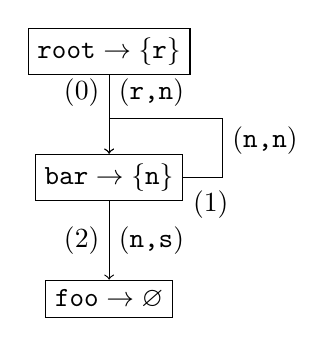
\begin{tikzpicture}[node/.style={rectangle, draw=black}]
            \node[node]  (foo)  {$\texttt{foo} \rightarrow \varnothing$};
            \node[node]  (bar) [above=of foo] {$\texttt{bar} \rightarrow \{\texttt{n}\}$};
            \node[node]  (root) [above=of bar] {$\texttt{root} \rightarrow \{\texttt{r}\}$};

            \draw[->] (bar) -- node[right] {$(\texttt{n,s})$} node[left] {(2)} (foo);
            \draw[->] (bar.east) node[right, yshift=-1em] {(1)} -| ($(bar.east) + (.5,.75)$) node[right, yshift=-.8em] {$(\texttt{n,n})$} -| (bar.north) ;
            \draw[->] (root) -- node[right, yshift=.8em] {$(\texttt{r,n})$} node[left, yshift=.8em] {(0)} (bar);
        \end{tikzpicture}
        \caption{Initial argument effect graph..}
        \label{fig:argument-effects-graph}
    \end{subfigure}

    \caption{Illustration of the argument effect graph (\ref{fig:argument-effects-graph}) of a simple Python program~(\ref{fig:argument-effects-code}).}
    \label{fig:argument-effects}

\end{figure}


%\subsection{Range Analysis}

\subsection{Constant Propagation and Loop Unrolling}

% Cette partie n'a pas déjà été écrite dans un autre papier?
%SG: non
There are very few values that are considered as constant in Python, to the
notable exception of strings and tuples. However there are a lot of constant
propagation opportunities, the most remarkable one being calls to the
\texttt{range} built-in with literal parameters.

A naive translation of such call to a generic C++ function would generate a
call to a C++ function that would allocate enough memory to hold three integers,
fill the corresponding buffer and return it. A smarter version would generate a
static array holding the relevant values. Figure~\ref{fig:unroll-range}
compares two translations of a Python snippet that iterates over a fixed-size
list. The Clang compiler successfully turns Listing~\ref{lst:stat} into a
single constant. It also statically computes the return value for
Listing~\ref{lst:dyna}, but still generates the initialization code for the
\texttt{std::vector}. The GCC compiler fails to statically compute the return
value in both cases. This example shows that constant propagation should be
done at a higher level than C++, and so be part of the Python optimizer.

The argument effect analysis described in \S~\ref{sec:fs} can be extended to
global variables to determine if a function has side effects on its arguments or
on global variables (including I/O). This information makes it possible to flag
some function as pure, and to statically evaluate pure function calls with
constant arguments. This evaluation is especially feasible in Python thanks to
the ability of the language to turn an AST expression into bytecode, evaluate it
and retrieve its constant value. For instance, this makes it possible to turn a
call to \texttt{range(3)} into \texttt{[0, 1, 2]}, but also to compute the
value of \texttt{fibonnaci(4)} at compile-time.


\begin{figure}

    \begin{subfigure}{.5\textwidth}
    \begin{lstlisting}[language=python]
s = 0
for i in [0,1,2]:
    s += i
return s
\end{lstlisting}
\caption{Python version.}
\end{subfigure}

    \begin{subfigure}{.5\textwidth}
\begin{lstlisting}[language=c++]
long s = 0;
for(auto i: std::vector<long>{{0,1,2}}:
    s += i;
return s;
\end{lstlisting}
\caption{C++ version with dynamic allocation.}
\label{lst:dyna}
\end{subfigure}

    \begin{subfigure}{.5\textwidth}
\begin{lstlisting}[language=c++]
long s = 0;
for(auto i: std::array<long, 3>{{0,1,2}}:
    s += i;
return s;
\end{lstlisting}
\caption{C++ version with static allocation.}
\label{lst:stat}
\end{subfigure}
% Hum, on dirait du pattern transform : list => tuple pour l'iterable du for

    \caption{Different implementations of an iteration over a fixed size container.}
    \label{fig:unroll-range}

\end{figure}

Once interprocedural constant evaluation is done (eventually followed by
forward substitution), iteration over fixed size lists may be exposed, giving an
opportunity to fully unroll these loops at the Python level, thus avoiding the
suboptimal C++ translation observed for Listing~\ref{lst:stat}
and~\ref{lst:dyna}.

\subsection{Parallelization and Vectorization}

A simplified version of the evaluation loop for an expression template is
illustrated on Listing~\ref{lst:eval-et}. The loop over each dimension of the
target array expression \texttt{to} is made explicit through a recursive
template call. The computation of the \texttt{from} expression is only triggered
for the innermost loop.

By construction of the expression template, the \texttt{eval} method used in
\texttt{from.eval(i)} does not have side effects, and the Python to C++
compiler can assert there is no shared memory between \texttt{to} and any
component of \texttt{from}. In that case, all loops can be made parallel, and
the innermost loop is eventually vectorizable.

\begin{lstlisting}[language=c++, label={lst:eval-et}, caption={Evaluation body of an expression template}]
template<size_t N> struct D {};

// real evaluation loop
template<class A, class E>
void eval(A& to, E const& from, D<1>)
{
  size_t n = to.shape[A::ndims-1];
  for(size_t i = 0; i < n; ++i)
    to[i] = from.eval(i);
}

// recursive evaluation loops
template<class A, class E, size_t Dim>
void eval(A& to, E const& from, D<Dim>)
{
  size_t n = to.shape[A::ndims-Dim];
  for(size_t i = 0; i < n; ++i)
    eval(to[i], from[i], D<Dim-1>);
}
\end{lstlisting}

\subsubsection{Parallelization of Expression templates}

A naive way to parallelize the parametric loop nest from
Listing~\ref{lst:eval-et} is to use a \texttt{parallel} directive from the
OpenMP~\cite{openmp4} standard. Depending on the number of dimensions of the
input array, this may lead to nested parallel regions. When OpenMP nested
parallel regions are activated, each parallel region spawns as many threads as
possible up to the runtime upper bound, which leads to oversubscription with
more common implementation (libgomp and libiomp) and generally bad performances. When
disabled, only the first parallel region spawns threads, which is likely to be
inefficient depending on the input array shape, e.g. $(1,100000)$. Moreover,
even if they do not start new threads, each nested parallel region implies a
costly overhead for scheduling computation and data sharing. An easy way to solve
the issue with small then large dimension is to use the \texttt{collapse}
clause but it is not compatible with the parametric loop version.

%A first approach would be to use recursive tasks and manual loop chunking.
%\todo{pierrick ? c'est bête comme idée ?}
% Les taches sont en général plus lente que les boucles for (malheureusement)
% et il y a des fois ou on ne pourra jamais être plus rapide si on passe par
% des taches.
% Souvent, c'est a cause du scheduling static qui permet d'optimiser le cache
% et aussi parce que les compilos, quand ils voient un omp for static, ils
% font directement du déroulage de boucle. (Jusqu'au full unrolling des fois
% avec autant de tache que de thread).
%
% Dans notre cas, on ne connait pas forcement la taille de l'espace d'iteration
% a la compilation. On ne pourra donc pas faire trop de unrolling mais bon, on
% doit pouvoir faire comme gcc. Par contre, pour l'optimisation du cache, les
% boucles for assurent que c'est le même noeud qui exécute le même "chunk" entre
% les boucles for et ça, on le perd avec les taches. Je ne sais pas si ça joue
% vraiment.
% Autre problem. On va créé des taches en assez grande quantité. Ce que libgomp
% supporte assez mal. Aussi, on va créé du datasharing pour des petites taches
% (iteration de longueur 1 dans le cas du (1, 1000000)) ce qui est couteux et
% assez mal supporté par libgomp. Il faudra voir comment ça se passe avec libiomp
% qui est utilisé par clang.
%
% Au final : Ca doit être jouable. Il y a plusieurs raisons qui peuvent faire
% qu'on a de mauvaise perfs mais sans mesures, on ne sait pas.

A conservative approach is to only start a parallel region if the loop trip
count is large enough. We avoid by using the \texttt{if} clause for parallel
regions to do so in order to prevent the unnecessary overhead. Instead a manual
if is used: the loop statement is duplicated and guarded by the appropriate
check, where only one loop holds the parallel annotations.
\todo{this paragraph seems to be about a particular runtime issue, this shouldn't matter.
Moreover, how is it relevant to this paper? It is an "implementation detail"}

Note that this parallelization scheme is compatible with the manual
parallelization of Python programs proposed in~\cite{pyhpc2013}.
\todo{I think a specific section could be made on this topic}

\subsubsection{Vectorization of Expression Templates}

A first exploration of vectorization of Python constructs is done
in~\cite{wpmvp2014}. It shows that language constructs like list comprehension
offer many vectorization opportunities. This section focuses on the
vectorization of complex Numpy expressions. In order to vectorize a Numpy
expression, the last dimension of the expression must be contiguous. This can
be checked at compile time using type traits. The general form of a subscripted
array can be expressed in C++ using a template type, say \texttt{numpy\_gexpr}.
For instance the Numpy subscript \lstinline|a[:,0,::2]| on a 3D float matrix is
represented by the C++ type in Listing~\ref{lst:gexpr}.

\begin{lstlisting}[language=c++, caption={C++ type corresponding to the Numpy subscript \lstinline{a[:,0,::2]} on a 3D float matrix}, label={lst:gexpr}]
numpy_gexpr<ndarray<double, 3>,
            contiguous_slice,
            long, slice>
\end{lstlisting}

This representation makes it easy to
statically compute, in a vectorizable type trait, whether the last dimension of
a subscript is contiguous or not. It can be generalized to the other array
manipulations. BOOST.simd~\cite{esterie2012boost} provides a
machine-independant abstraction for vector operation and supports all the C99
math library. This abstraction helps to vectorize all Numpy binary and unary
functions and operators in Pythran's runtime.

The loop described in Listing~\ref{lst:eval-et} can be specialized using this
vectorizable type trait, to automatically vectorize the innermost loop whenever
it is legal. The choice is statically made at compile time.


%%
%%
\section{Experiments} \label{sec:xp}

\subsection{The Pythran Compiler}

The ideas described in this paper are implemented in the Pythran
compiler~\cite{pythran2013}, a translator from a subset of Python to
C++11~\cite{isocxx11}. The architecture of the compiler is briefly described
in Figure~\ref{fig:pythran-compiler}. The input is a Python module written in
the Pythran subset. Pythran translates it in its internal representation, a
simplified Python AST. It performs various optimization then outputs either
Python code, in a source-to-source fashion, or C++ template code that makes
call to the pythonic library that typically implements the \texttt{ndarray}
interface. User annotations can be used to instantiate this code for the proper
types and generate a native library. This library relies on Boost.Python
library to match Python's C API.

The Pythran compiler is an open source project publicly released under the BSD
license~\footnote{\url{http://pythonhosted.org/pythran/}}.

\begin{figure}

    \centering
    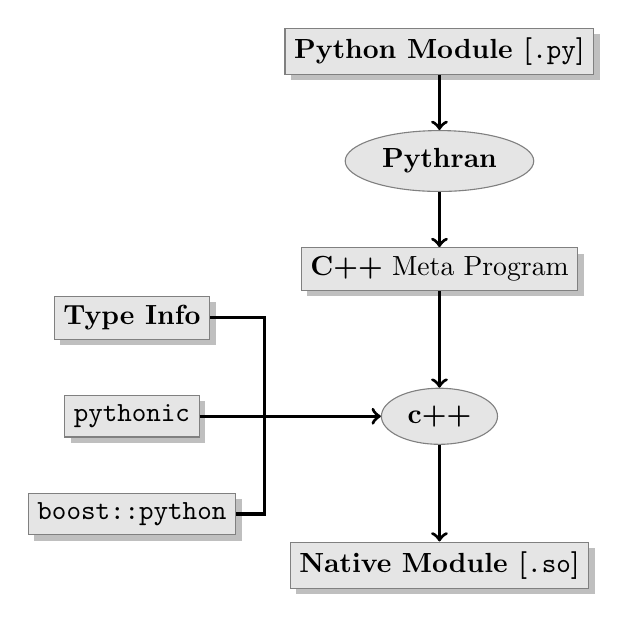
\begin{tikzpicture}[
            file/.style={draw=black!50,fill=black!10,rectangle, drop shadow, align=center,
            node distance=0.7cm},
            tool/.style={draw=black!50,fill=black!10,ellipse, align=center, node
        distance=0.7cm}]
        \node[file] (python) {\textbf{Python Module [\texttt{.py}]}};
        \node[tool] (pythran) [below=of python] {\textbf{Pythran}};
        \node[file] (meta-cxx) [below=of pythran] {\textbf{C++} Meta Program};
        \node[tool] (gxx) [yshift=-1.5em, below=of meta-cxx] {\textbf{c++}};
        \node (empty) [xshift=-1em, left=of gxx] {};
        \node[file] (pythonic) [left=of empty] {\textbf{\texttt{pythonic}}};
        \node[file] (annotation)     [above=of pythonic] {\textbf{Type Info}};
        \node[file] (boost) [below=of pythonic] {\textbf{\texttt{boost::python}}};
        \node[file] (so) [yshift=-1.5em, below=of gxx] {\textbf{Native Module [\texttt{.so}]}};

        \draw[very thick, ->] (python) -- (pythran);
        \draw[very thick] (annotation) -| (empty.center);
        \draw[very thick, ->] (pythran) -- (meta-cxx);
        \draw[very thick, ->] (meta-cxx) -- (gxx);
        \draw[very thick] (boost) -| (empty.center);
        \draw[very thick, ->] (pythonic) -- (gxx);
        \draw[very thick, ->] (gxx) -- (so);
    \end{tikzpicture}

    \caption{Pythran compilation flow.}
    \label{fig:pythran-compiler}

\end{figure}

\subsection{Experimental Setup}

As introduced in \S~\ref{sec:stackoverflow}, we use the numpy-benchmark test 
suite to evaluate the optimizations described in\S~\ref{sec:pythran}. 
Pythran is used (commit: 488b7ba) with and without SIMD optimization. 
The results are compared with Pypy (commit: 632c832bd32f), Parakeet (commit: 4e55810), 
Numba (commit: b8a79c5) and Python 2.7.

numpy-benchmarks run 11 times benchmarks with an execution time around 1 seconde.
THe best time, average time and standard deviation is return from these 11 runs.

Benchmarking is done on two architectures with different backend compilers.

The first one holds 8 AMD Magny Cours processors for a
total of 48 cores. Each core has access to 64\,KB of L1 cache,
512\,KB of L2 cache. Both L1 and L2 caches are private, while L3 cache
is shared between the 6 cores of a processor. This configuration
provides a total of 256\,GB (32\,GB per NUMA node) of main memory. It supports
up to SSE4. We refer to this configuration as \textbf{AMD48}.
On AMD48, the backend compilers is the clang-omp
version from intel~\footnote{\url{http://clang-omp.github.io/}} to be able to
benefits from OpenMP improvements. This Clang version is based on Clang 3.4
release (LLVM:233b1e3f034, clang-omp:6f358bcd87).

The second one holds one Intel(R) Xeon(R) CPU E5-2650 0 @ 2.00GHz for a total of
8 cores (multithreading is not used). Each node can access to 64\,KB of L1
cache, 256\,KB of L2 cache. Both L1 and L2 caches are private, while L3 cache
is shared between the 8 cores. This configuration provides a total of 64\,GB of 
main memory. It supports up to AVX. We refer to this configuration as
\textbf{Intel8}.
On Intel8, backend compilers is GCC 4.9 (20140528) with libgomp.


\subsection{Performance of the Rosenbrock Function}

% For performance comparison between different Pythran version
To compare the different optimization schemes, we run the numpy-benchmarks test
suite multiple times on the \textit{rosen} benchmark. The algorithm is the one
on Listing~\ref{lst:rosen} and input is a raw array of 1,000,000 double elements.
Figures~\ref{fig:rosenamd48} and \ref{fig:rosenintel8} illustrate the results.
The speedup difference between the two architectures can be explain by AVX support on
the Intel8 architecture while AMD48 supports up to SSE4 only.
We can also notice importance of forward substitution on this benchmarks as
we avoid extra loop, 2 temporary array assignment and avoid some load/store for
SIMD instructions.

\begin{figure}[t]
\centering
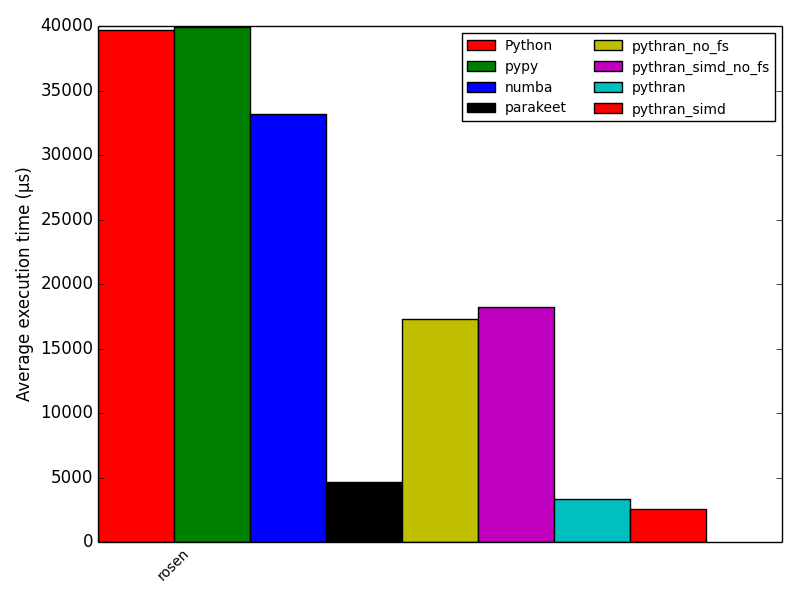
\includegraphics[width=0.5\textwidth]{rosen_amd48.png}
\caption{Execution time of the rosen kernel on AMD48.}
\label{fig:rosenamd48}
\end{figure}

\begin{figure}[t]
\centering
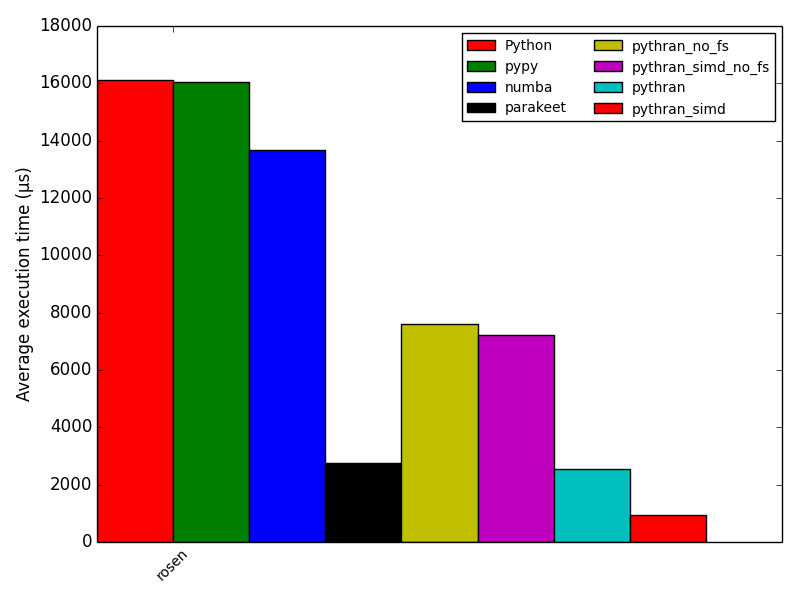
\includegraphics[width=.5\textwidth]{rosen_intel8.png}
\caption{Execution time of the rosen kernel on Intel8.}
\label{fig:rosenintel8}
\end{figure}


\subsection{Comparison with others Python compiler}


Table~\ref{tbl:overview} presents the average execution time for each kernel
and each compiler, with the lowest values highlighted in
bold font. Zeros are used when the given compiler failed to
compile the kernel. Concerning the Numba compiler, this
benchmarks confirms that it works best on explicit loops. It
gives non performance gain when run on high-level kernels,
either falling back to the generation of calls to Python C
API, or stopping compilation. PyPy is the most robust of
the compilers, but to a few exceptions, it does not generate
code more efficient than the original version. This reflects
the fact that Numpy support is still a work-in-progress task.
Parakeet performs extremely well on high-level benchmarks.
Although it does not supports some Numpy constructs, it
successfully parallelize many of them, and also generates
efficient code for explicit loops. Pythran still performs better
than Parakeet on some kernels, whenever it successfully
vectorizes operations.

\begin{table*}

    \centering{
\begin{tabular}{|l||c|c|c|c|c|}
\hline
& Python & numba & parakeet & pypy & pythran \\
\hline
\hline
         allpairs\_distances &   58293 &             0 &          3170 &   59232 & \textbf{1583} \\
  allpairs\_distances\_loops &   64137 &         72748 &          3158 &   65287 & \textbf{3146} \\
               arc\_distance &    2796 &          2792 &          3084 &    2791 &  \textbf{103} \\
                        conv & 3260079 &             0 & \textbf{3284} & 3268298 &          3420 \\
                create\_grid &    5231 & \textbf{5044} &             0 &    5240 &          5587 \\
                    cronbach &    1905 &          2016 &             0 &    1909 & \textbf{1890} \\
                   diffusion &   42998 &         45030 & \textbf{8843} &   43238 &         21704 \\
                      evolve &    8236 &             0 &             0 &    8319 & \textbf{6242} \\
                        fdtd & 1940884 &       1498849 &             0 & 2007839 & \textbf{2294} \\
                         fft &   27120 &             0 &             0 &   27009 & \textbf{2151} \\
                    grouping &    3739 &             0 &             0 &    3740 & \textbf{1747} \\
                     growcut & 2112332 &         11617 & \textbf{5485} & 2141571 &         10338 \\
                      harris &    7173 &          9116 & \textbf{4240} &    7322 &          4889 \\
                     hyantes &  288852 &             0 & \textbf{2834} &  289074 &          3522 \\
                       julia & 1744357 &          5168 &  \textbf{109} & 1771329 &          4255 \\
                      l2norm &    5966 &          5948 &          9210 &    6559 &  \textbf{551} \\
               local\_maxima &  132237 &             0 &             0 &  132047 & \textbf{8561} \\
                      lstsqr &    9254 &          7528 &             0 &    8992 & \textbf{1414} \\
                      mandel &  951612 & \textbf{8175} &             0 &  951687 &         10341 \\
               multiple\_sum &    5477 &          5813 &          9805 &    5475 & \textbf{3503} \\
                    pairwise & 3362150 &         10764 &          6199 & 3347574 & \textbf{6015} \\
              periodic\_dist &    2559 &          2675 &             0 &    2562 & \textbf{2292} \\
                   repeating &    2808 &          2836 &             0 &    2795 &  \textbf{810} \\
             reverse\_cumsum &    4583 &          4828 &             0 &    4583 & \textbf{2379} \\
                       rosen &   15382 &         14309 &          2763 &   16065 &  \textbf{939} \\
                   slowparts &    8302 &             0 & \textbf{1610} &    8241 &          1927 \\
                   smoothing &  834057 &          8478 &          9771 &  819827 & \textbf{8254} \\
             specialconvolve &   12537 &         11978 &          6039 &   12570 & \textbf{5572} \\
                vibr\_energy &    5277 &          5275 &          5334 &    5416 &  \textbf{146} \\
                        wave &   72394 &         67590 &             0 &   72300 & \textbf{5186} \\
                       wdist &  108572 &        119211 &          4197 &  108283 & \textbf{4010} \\
\hline
\end{tabular}
}
\caption{Average execution times for all kernels of the numpy-benchamrks on Intel8 with OpenMP (8 threads) and SIMD extension.}
\label{tbl:overview}
\end{table*}


Figure~\ref{fig:arc_distance} and \ref{fig:arc_distance_intel8} are typicals
example where we can make intensive
use of the techniques described in this paper. It shows speedup compare to one
thread execution for the arc\_distance benchmark.This kernel performs intensive
points to points computation and trigonometrics use. We can see that OpenMP
improvement is scalable up to 20 threads with a raw array of 10,000,000 double
elements as input.

\begin{figure}[t]
\centering
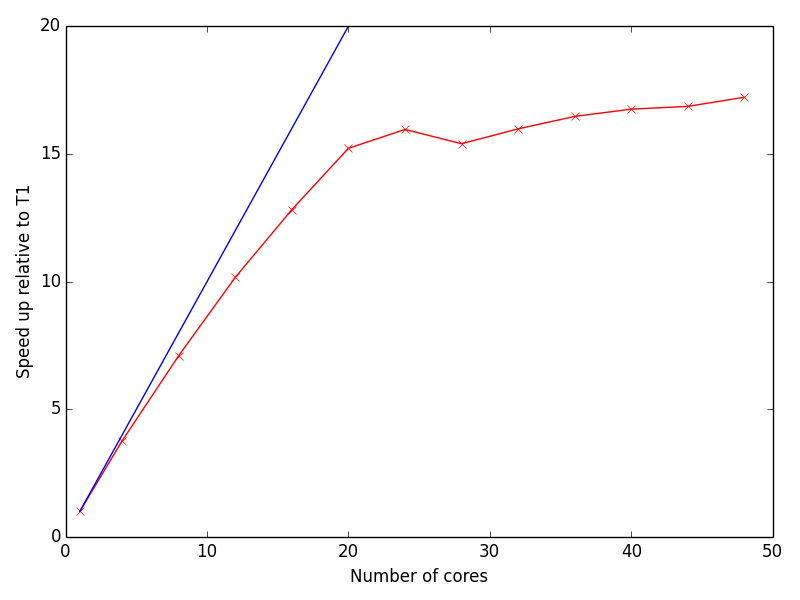
\includegraphics[width=0.5\textwidth]{arc_distance_amd48.png}
\caption{Speed up for the arc distance kernel on AMD48.}
\label{fig:arc_distance}
\end{figure}

\begin{figure}[t]
\centering
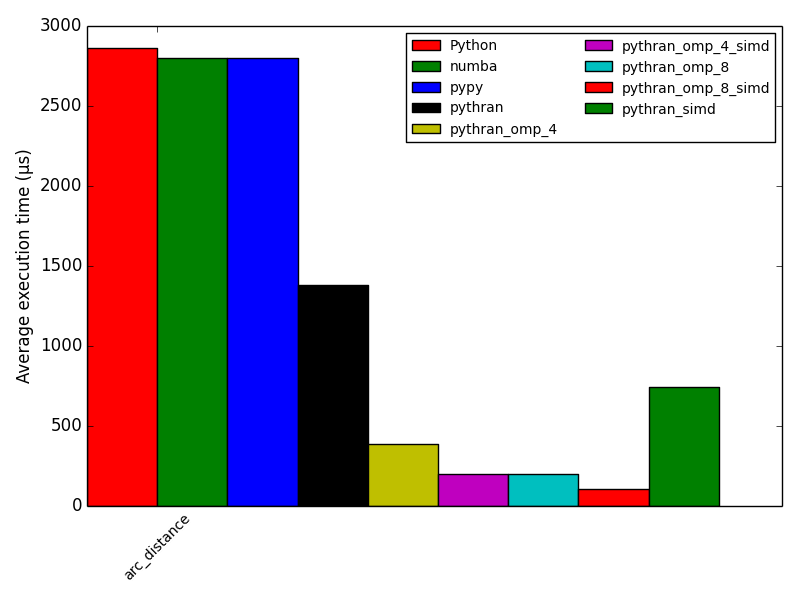
\includegraphics[width=0.5\textwidth]{arc_distance_intel8.png}
\caption{Speed up for the arc distance kernel on Intel48.}
\label{fig:arc_distance_intel8}
\end{figure}

Finally, Figure~\ref{fig:l2norme} and \ref{fig:l2norm_intel8} shows the L2norm algorithm introduced in
\S~\ref{sec:stackoverflow}. Comparison with other compilers illustrates how the
approach taken by Pythran is relevant for these kind of functions. Just like for
the arc\_distance benchmarks, we can notice use of AVX when it is available.

\begin{figure}[t]
\centering
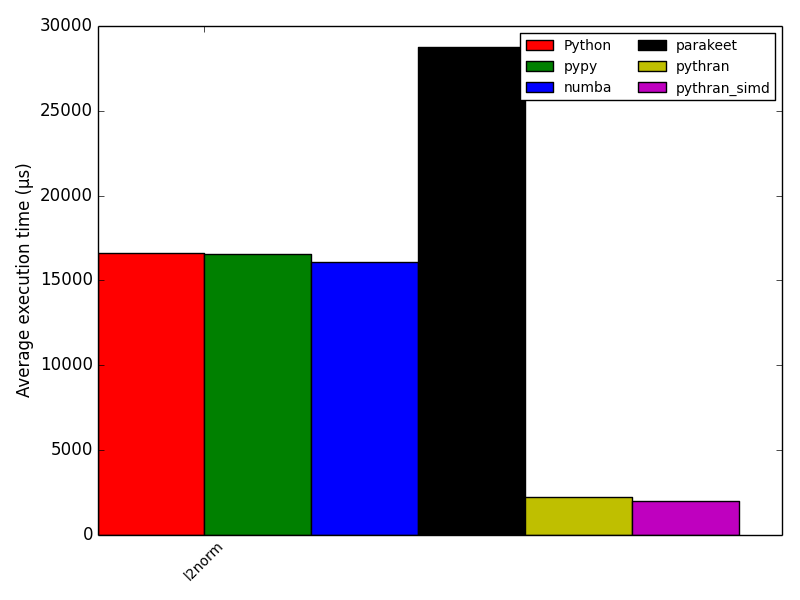
\includegraphics[width=0.5\textwidth]{l2norm_amd48.png}
\caption{Execution time of the l2norm kernel on AMD48.}
\label{fig:l2norme}
\end{figure}

\begin{figure}[t]
\centering
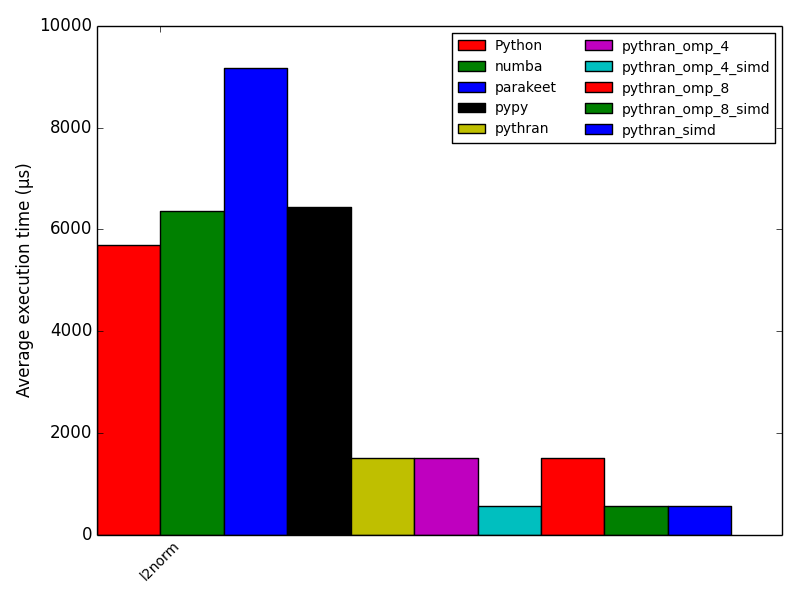
\includegraphics[width=0.5\textwidth]{l2norm_intel8.png}
\caption{Execution time of the l2norm kernel on Intel8.}
\label{fig:l2norm_intel8}
\end{figure}


%%
%%
\section*{Conclusion}

\acks

The Pythran project is an independent Open Source initiative that has been
partially funded by the CARP Project and the SILKAN Company.

Several Students of Télécom Bretagne, namely Adrien Merlini, Alan Raynaud,
Xavier Corbillon, Yuancheng Peng and Eliott Coyacc, have made significant
contributions to the project.

% We recommend abbrvnat bibliography style.

\bibliographystyle{abbrvnat}
\bibliography{biblio}


\end{document}
